\section{Split Class Reference}
\label{classSplit}\index{Split@{Split}}
Inheritance diagram for Split:\begin{figure}[H]
\begin{center}
\leavevmode
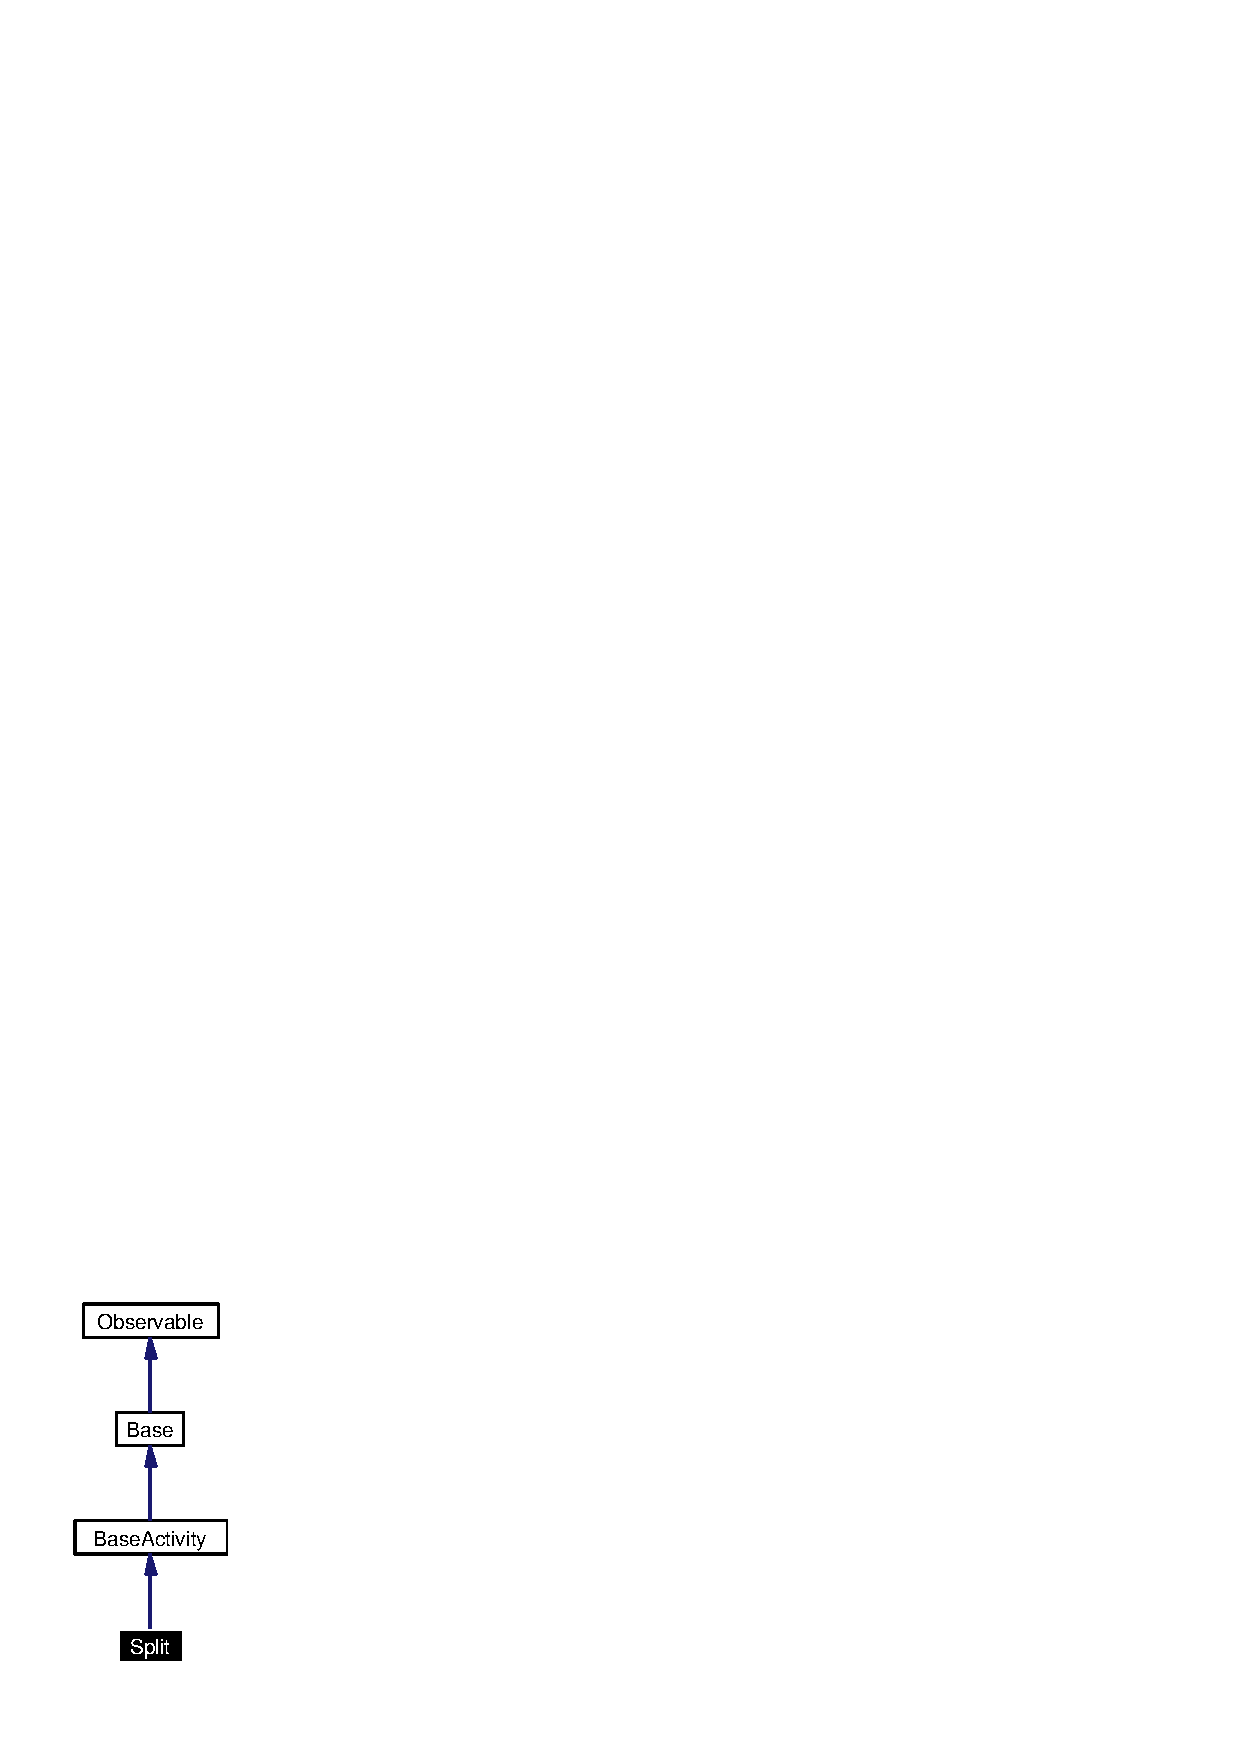
\includegraphics[width=54pt]{classSplit__inherit__graph}
\end{center}
\end{figure}
Collaboration diagram for Split:\begin{figure}[H]
\begin{center}
\leavevmode
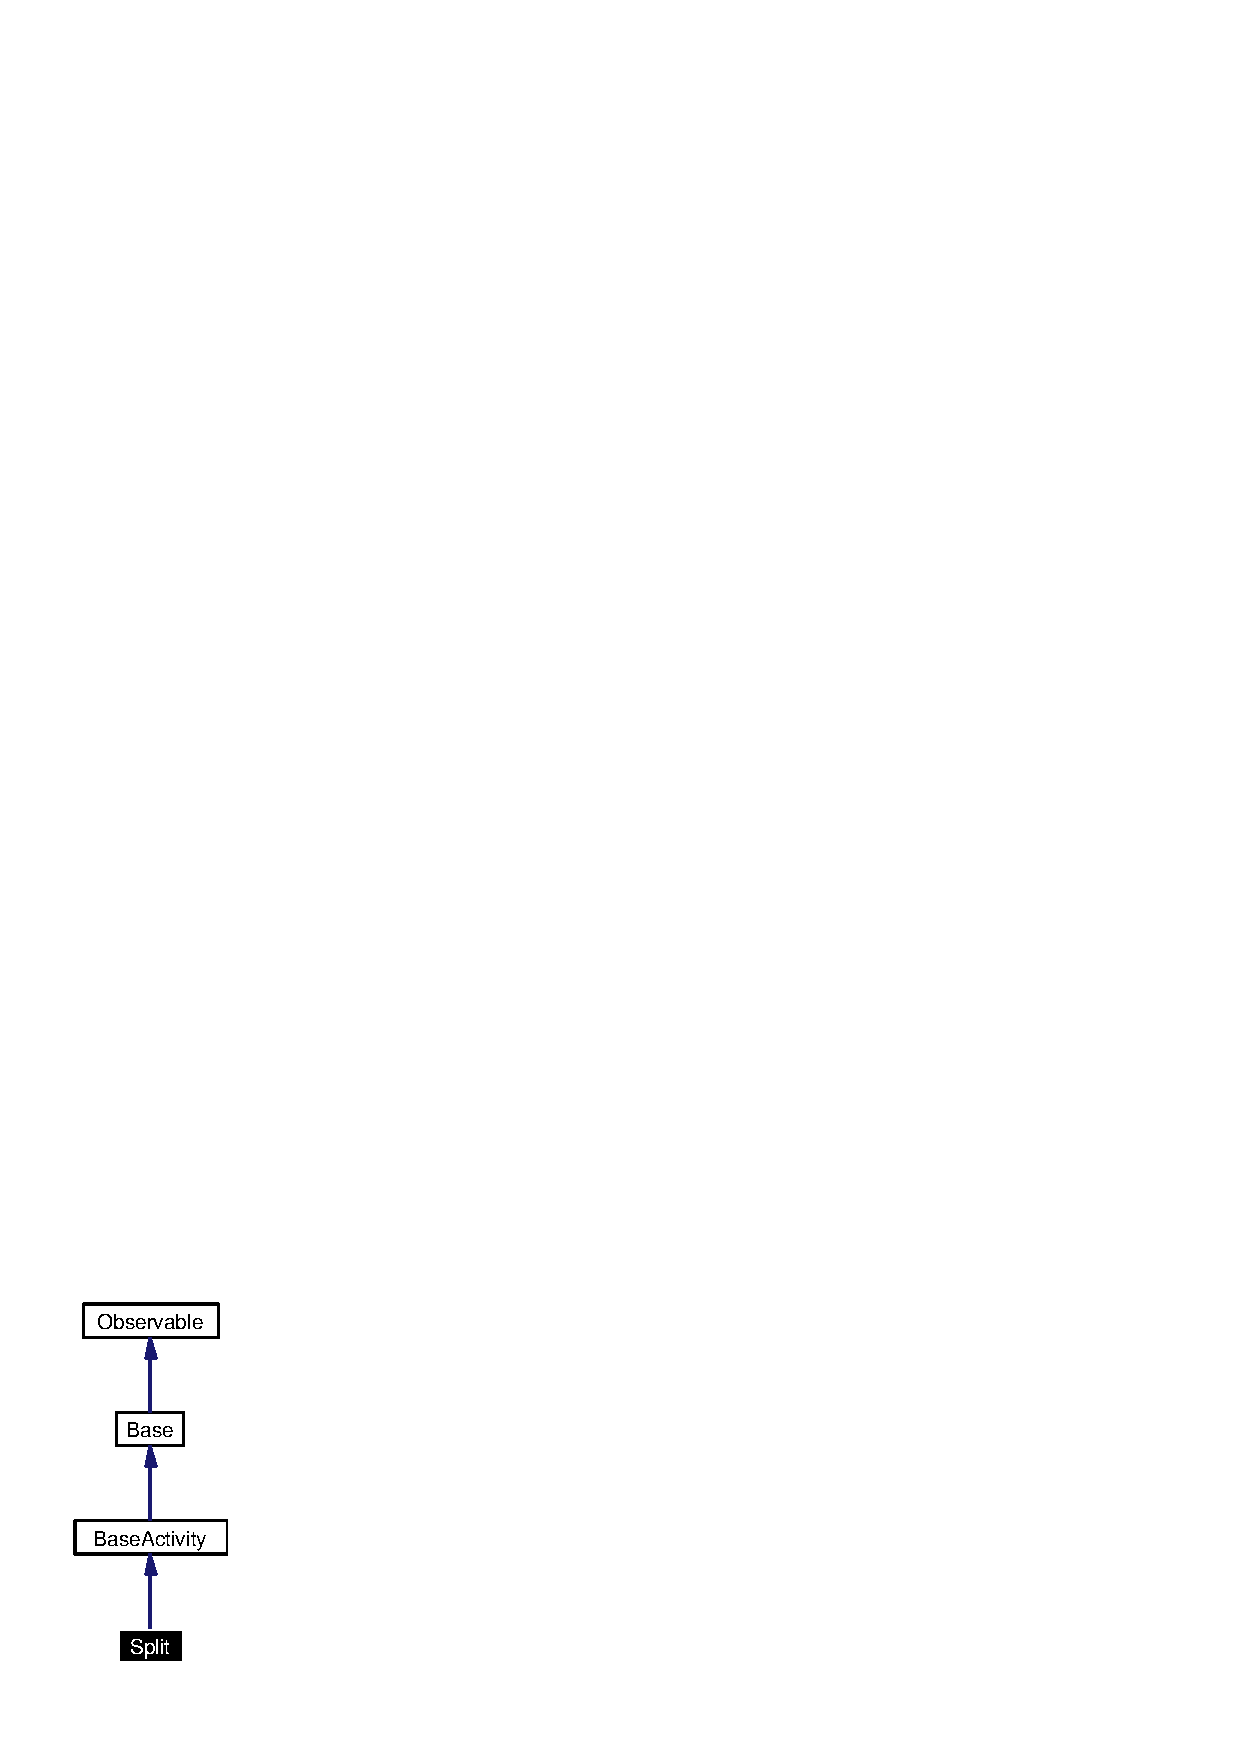
\includegraphics[width=54pt]{classSplit__coll__graph}
\end{center}
\end{figure}
\subsection*{Public Member Functions}
\begin{CompactItemize}
\item 
{\bf Split} (\$db)\label{classSplit_a0}

\end{CompactItemize}


\subsection{Detailed Description}
This class handles activities of type 'split' 



Definition at line 8 of file Split.php.

The documentation for this class was generated from the following file:\begin{CompactItemize}
\item 
Split.php\end{CompactItemize}
